\documentclass{article}
\usepackage[english]{babel}
\usepackage[utf8]{inputenc}
\usepackage{listings}
\usepackage{color}
\usepackage{algorithm}
\usepackage{algorithmic}
\usepackage{caption}

\usepackage{graphicx}
\usepackage{caption}
\usepackage{subcaption}
\usepackage{float}
\usepackage{tikz}
\usepackage{bbm}
\usepackage{todonotes}
\usepackage{siunitx}
\graphicspath{ {.} }


\newtheorem{theorem}{Theorem}

\definecolor{dkgreen}{rgb}{0,0.6,0}
\definecolor{gray}{rgb}{0.5,0.5,0.5}
\definecolor{mauve}{rgb}{0.58,0,0.82}

\lstset{frame=tb,
  language=Java,
  aboveskip=3mm,
  belowskip=3mm,
  showstringspaces=false,
  columns=flexible,
  basicstyle={\small\ttfamily},
  numbers=none,
  numberstyle=\tiny\color{gray},
  keywordstyle=\color{blue},
  commentstyle=\color{dkgreen},
  stringstyle=\color{mauve},
  breaklines=true,
  breakatwhitespace=true,
  tabsize=3
}

\title{BitTensor: An Intermodel Intelligence Measure}

\begin{document}






\section{Experiments}

\textbf{Ranking Accuracy} We use the empirical model in section 4.3 and draw multiple samples from $\theta$, solving for the competitive nash-equilibrium. We then calculate the coordinated ranking scores via the equation in section 2.3 and measure the spearman-rho coefficient between the two rankings. In the competitive convergence we use a learning rate of 0.001 for 10000 steps. The results for various terms $\alpha$ and $T$ are show in graph (?). 
\smallskip

\textbf{Price of Anarchy} We use the empirical model in section 4.3 and pull samples from the distribution over potential network configurations. We then measure the Price of Anarchy, a game-theoretic measure of efficiency in the system between equilibrium found during a coordinated and comeptitive setting. We report the change in Price of Anarchy for various network sizes and ranges of alpha. The results are shown in figure 2.
\smallskip

Without access to the parameters of each model we cannot guarantee that weights are being set honestly according to the method described in section 2.3. We assume instead, that  participants are self-interestedly attempting to maximize their subjective payoff. We define $P: R_n_\times_n \rightarrow R_1$, a measure of how much value a participant attains from each choice of weights. This can be described by two terms (a) the utility attached to their loss $U(\mathcal{L}(W)))$ (via section 2) and (b) the revenue attained via token emission $E(\tau(W))$ (via section 3). Without loss of generality these are measured in similar units:
\smallskip


\[ \textrm{P}(W) = U(\mathcal{L}(W)) \ + \ E(\tau(W)) \] 

At each iteration $t$, each participant is competitively submitting, potentially null changes, to their row of weights $\Delta w_i = [\Delta w_{i_0}, ..., \Delta w_{i, n}]$, and attempting to maximize their payoff. The payoff is full differentiable w.r.t to the weights $\frac{\partial P}{\partial w_i} = \frac{\partial \mathcal{L}}{\partial w_i} + \frac{\partial E(\tau(W))}{\partial w_i}$, and we prove in the appendix that the strategy which achieves \textit{zero expect ex-post regret}: namely, the strategy which does at least as well as any other strategy in expectation under a sufficiently small learning rate, is the strategy which makes gradient steps $\Delta w_i = \lambda * \frac{\partial P}{\partial w_i}$ during every iteration.
\smallskip

We use the zero-regret strategy to analyze the behaviour of the system. To do this, we set the at each iteration we produce a gradient step $\Delta W = [\frac{\partial P}{\partial w_0}, ..., \frac{\partial P}{\partial w_n}]$ and apply it to the weights. The ranking found by this competitive process is found the one converged to at equilibrium: the point where no participant can make changes to their weights and improve their payoff.

Above, the $\alpha$ term is the maximum change in the utility w.r.t to the loss a constant which is always negative in the change in loss at the minimum. i.e. $\alpha$ lower-bounds the maximum and the $H(L)$ term is the same hessian of the loss described in section 2.3. We can see from above that each instantiation of the network can parameterized by $\theta = [\alpha, H]$.
\maketitle

\begin{abstract}

A purely inter-model version of a machine intelligence benchmark would allow us to measure intelligence directly as information without projecting that information onto labeled datasets. In the proposed framework other learners score the informational significance of their peers across a network and use a digital ledger to negotiate the global ranks. However, the main benefits of measuring intelligence with other learners are lost if the underlying scores are dishonest. As a solution, we show how competition for connectivity in the network can be used to force honest bidding. To make this claim we prove that selecting inter-model scores using gradient descent is a regret free strategy; one which generates the best subjective-outcome regardless of the behaviour of others. We then empirically show that when nodes apply this strategy the network converges to a ranking which correlates with the one found in a fully coordinated and centralized setting. The result is a fair mechanism for training an internet wide, decentralized and incentivized machine learning system, one which produces, on an ongoing basis, a continually hardening and expanding benchmark at the generalized intersection of the participants.

\end{abstract}

\section{Introduction}

Machine intelligence has come to rely almost entirely on benchmarks --- scores on labelled datasets -- as a feedback signal for the field globally. While benchmarks provide a clear and human interpretable, they are incapable of measuring the -resolution proxies for the intelligence, .  Specifically, the salient element to improve in fields such as image and language understanding are the semantic, causal, disjoint representations of inputs, rather than the benchmark scores on a small set of supervised tasks. Canonical benchmarks like GLUE only measure performance on 10 distinct tasks for instance, which is a proxy-measure for the conceptual understanding of the much higher dimensional representations learnt by models, like BERT or GPT-2, which it evaluates. Such a collapse losses the unique distributional knowledge encoded by the model, i.e. Hinton's 'Dark Knowledge', and subsequently misses models which may have improved it. For instance, those that cover regions disjoint from those evaluated by the benchmark, or those which generalized across the entire domain but performed worse on the specific. By narrowing the avenue of reward, small-research teams cannot focus on niche areas of improvement within the larger problem. Those that succeed must have the major computational power to compete with the largest corporations. 
\smallskip

What is needed is a method of rewarding learning systems by measuring their intelligence contribution at the informational level. The proposal in this paper, is to measure contributions via other learners in an inter-model system. Learners rank each other, not by projecting the learned representations onto labels, but by measuring the informational content their peers create. We design the benchmark to run in an continuous, asynchronous fashion, peer to peer, across the internet such that any number of supervised or unsupervised tasks, or any number of computers can be concurrently added to the system. The models are connected and are learning from each other, sharing the knowledge produced by one with the rest, compounding what has been learned before and expanding the corpus of knowledge within the domain. 
\smallskip

\section{Method}

\subsection{Objective}

We define the benchmark to run over $n$ parameterized functions $F = {f_0, ...,  f_j, ...f_n}$ where each function is producing an output tensor $f_i(F(x))$, a 'representation', from an input tensor $F(x) = [f_0(x) ... f_n(x)]$ gathered by querying its neighbors. The benchmark objective is defined by these participants, where each is actively training over a dataset $D_i=[X,Y]$, such that, given an error function $Q_i$, its expectation over that data $E_D_i$ defines a loss $\mathcal{L}_i$.
\bigskip

\[ \mathcal{L}_i = \  E_D_i[Q_i( \ y, \ f_i(F(x)) \ )]  \ \ \ \  \textrm{ } \]


\begin{figure}[H]
    \centering
    \hspace*{-2cm}
    \begin{center}
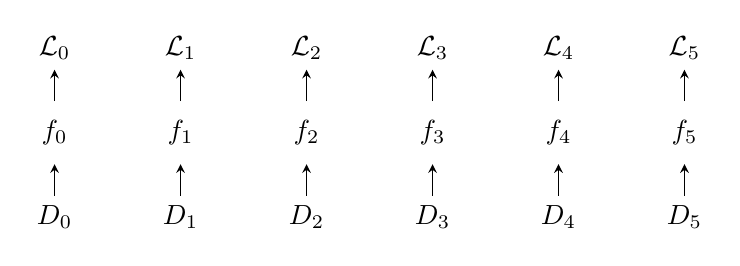
\begin{tikzpicture}
\begin{scope}[scale=0.8]
    
    
    \node (a) at (0,0) [rectangle, rounded corners] {$f_0$};
    \node (b) at (2,0) [rectangle, rounded corners] {$f_1$};
    \node (c) at (4,0) [rectangle, rounded corners] {$f_2$};
    \node (d) at (6,0) [rectangle, rounded corners] {$f_3$};
    \node (e) at (8,0) [rectangle, rounded corners] {$f_4$};
    \node (f) at (10,0) [rectangle, rounded corners] {$f_5$};
    
    \draw[-stealth] (0,0.5) -- (0, 1) node[above] {$\mathcal{L}_0$};
    \draw[-stealth] (2,0.5) -- (2, 1) node[above] {$\mathcal{L}_1$};
    \draw[-stealth] (4,0.5) -- (4, 1) node[above] {$\mathcal{L}_2$};
    \draw[-stealth] (6,0.5) -- (6, 1) node[above] {$\mathcal{L}_3$};
    \draw[-stealth] (8,0.5) -- (8, 1) node[above] {$\mathcal{L}_4$};
    \draw[-stealth] (10,0.5) -- (10, 1) node[above] {$\mathcal{L}_5$};

    
    \draw[-stealth] (0, -1) node[below] {$D_0$} -- (0, -0.5);
    \draw[-stealth] (2, -1) node[below] {$D_1$} -- (2, -0.5);
    \draw[-stealth] (4, -1) node[below] {$D_2$} -- (4, -0.5);
    \draw[-stealth] (6, -1) node[below] {$D_3$} -- (6, -0.5);
    \draw[-stealth] (8, -1) node[below] {$D_4$} -- (8, -0.5);
    \draw[-stealth] (10, -1) node[below] {$D_5$} -- (10, -0.5);
    
\end{scope}
\end{tikzpicture}
\end{center}

    \label{fig:progdense_diagram}
    \caption{n=5 parameterized functions with losses $\mathcal{L}_i$ and datasets $D_i$.}
\end{figure}{}

\subsection{Inter-ranking}

Our goal is to measure intelligence contribution to the entire benchmark by producing ranks for each component $r_i \in R_n$. This is achieved by gathering a set of inter-model contribution weights --- scores attributed to a model from its peers --- into a $n \times n$ square matrix $W$, where each row sums to 1, $||w_i||_1 = 1$ and the weight $w_{i,j}$ is the score attributed to $f_j$ from $f_i$. We then produce a ranking for each component by taking the column sum. 
\bigskip

\[ R = W^T * \mathbbm{1}  \]

 \begin{figure}[H]
    \centering
    \hspace*{-2cm}
    \begin{center}

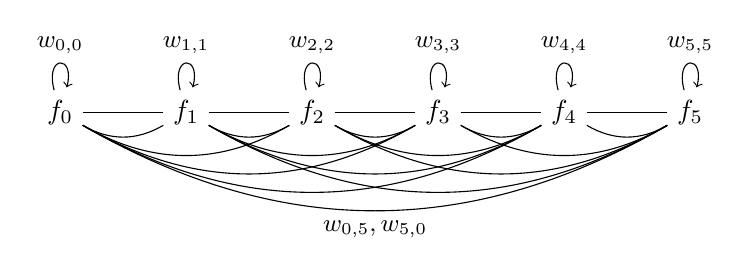
\begin{tikzpicture}


\begin{scope}[scale=0.8]

    \node (a) at (0,0) [rectangle] {$f_0$};
    \node (b) at (2,0) [rectangle] {$f_1$};
    \node (c) at (4,0) [rectangle] {$f_2$};
    \node (d) at (6,0) [rectangle] {$f_3$};
    \node (e) at (8,0) [rectangle] {$f_4$};
    \node (f) at (10,0) [rectangle] {$f_5$};
    
  
    \path[every node/.style={font=\sffamily\small}]
        (a) edge node [right] {} (b)
        (b) edge node [right] {} (c)
        (c) edge node [right] {} (d)
        (c) edge node [right] {} (d)
        (d) edge node [right] {} (e)
        (e) edge node [right] {} (f)


        (a) edge [loop above]  node[above]  {$w_{0,0}$} (a)
        (b) edge [loop above]  node[above]  {$w_{1,1}$} (b)
        (c) edge [loop above]  node[above]  {$w_{2,2}$} (c)
        (d) edge [loop above]  node[above]  {$w_{3,3}$} (d)
        (e) edge [loop above]  node[above]  {$w_{4,4}$}  (e)
        (f) edge [loop above]  node[above]  {$w_{5,5}$}  (f)

        (a) edge [bend right]  (b)
        (a) edge [bend right]  (c)
        (a) edge [bend right]  (d)
        (a) edge [bend right]  (e)
        (a) edge [bend right]  node[below]  {$w_{0,5}, w_{5,0}$}(f)
        (b) edge [bend right]  (c)
        (b) edge [bend right]  (d)
        (b) edge [bend right]  (e)
        (b) edge [bend right]  (f)
        (c) edge [bend right]  (d)
        (c) edge [bend right]  (e)
        (c) edge [bend right]  (f)
        (d) edge [bend right]  (e)
        (d) edge [bend right]  (f)
        (e) edge [bend right]  (f);
    
\end{scope}


\end{tikzpicture}
\end{center}

    \label{fig:progdense_diagram}
    \caption{Inter-model contribution weights: $w_{i,j}$ the score attributed to $f_j$ from $f_i$}
\end{figure}{}

Here, $\mathbbm{1}$ is the $n \times 1$ vector of all ones which when multiplied by the matrix $W^T$ computes the column sum and returns a $n \times 1$ vector of ranks. The ranks are produced continuously, where at each step components are able to make small iterative changes to their row of weights $\Delta w_i$ with learning rate $\lambda$,

\[ W^t^+^1 = W^t + \lambda \Delta W \].

\subsection{Information Scores}

A measure of informational significance which is relevant to intelligence systems is the pruning score, or, specifically the change in loss induced by the removal of each node from the network. Following Le Cunn and others, the weights which reflect these pruning scores can be computed as follows
\bigskip


\[ w_i = max_w_i \ \ [ \sum_{x \in D} \Delta F(x)^T * H (\mathcal{L}) * \Delta F(x) ] \ \ s.t \ \  ||w_i||_1 = 1 \]

\bigskip

\[ \Delta F (x) = -F(x) \circ w_i = [-f_0(x) * w_i_0, ..., -f_n(x) * w_i_n] \]


Where $H(\mathcal{L})$ is the semi-definite hessian of the loss $\mathcal{L}$, then the weights which maximized this function are those which would induce the largest increase in loss under the change in inputs $-F(x) \circ w$. Similar scores are used in various pruning methods for neural networks. When $Q$ is the cross entropy $H(\mathcal{L})$ is an estimate of the Fishers information. The score can be empirical computed with little extra cost on the backward pass of the gradient.
\bigskip

While the scores produced by this method would reflect the informational significance of peers in the network if honestly computed, the computation is non-auditable in our distributed setting and it is reasonable to assume participants will select weights to artificially increase their own rank at the expense of than others. Moreover, since the network remains open, nodes may instead choose to create many spuriously neighbors and rank themselves higher. 
\bigskip


\subsection{Stake}

The proposed solution begins by introducing a finite resource $s_i \in S$, a component's 'stake' in the system, and an inflation mechanism $\tau$ which translates the ranking vector $R$ into additional stake as incentive. 
\bigskip

\[ R = W \circ S * \mathbbm{1} \] 

\[ S^t^+^1 = S^t + \tau (R) \] 

The $\circ$ here is the Hadamard product between the $n \times n$ matrix $W$ and the $n \times n$ matrix containing $S$ for each column, and $t$ is the same time step referred to in section 2.2. Stake serves two purposes: (1) since it is finite, new computers cannot spuriously create nodes to game the ranking and (2) the resource provides mechanism power. By providing it to nodes with large rank, this ensures that those with weight must have worked to attain it, or indirectly subsidized those who have done so already.

\subsection{Competitive weights}

Our proposal for ensuring weight accuracy begins by introducing competition for connectivity between components. The competitive mechanism uses a continuous differential activation function $\sigma$ with range $(0,1)$ and shift term $\mu_j$ which masks the outputs from one component to another:
\bigskip

\[\sigma =  \frac{1}{ 1 + e^-^\frac{x}{T}} \]

\[\Delta F_w_i = F \circ \sigma(w_i, \mu) = [f_0 \ \ ... \ \ f_n] \circ [\sigma(w_{i,0} - \mu_0) \   ... \ \ \sigma(w_{i,n} - \mu_n)] \]

For shift term at component $j$ we use the average of the weights in each column $\mu_j = (\frac{1}{n}) \sum_{i}^{n}{w_{i,j}}$, and the activation function is the temperature scaled sigmoid. Both activation and shift function are standards across the network. The differentiability of the activation is key since it enables computation of both $\frac{\partial L}{\partial W}$ and $\frac{\partial R}{\partial W}$. 

\subsection{Conditional computation}

Components employ a Sparsely-Gated Mixture-of-Experts (SGMoE) layer at the input. The gating layer determines a sparse combination of children to query for each example and then re-joins them using the the gating weights $g_j(x)$. The combined gated inputs are fed as input to the local function: 

\[f_i = f_i(G(x)) \ \ \ \  \textrm{ }\]

\[ G(x) = [ ..., g_j(x) * f_j(x), ...] \]

The layer cuts outward bandwidth using a parameter $k$ and is trainable w.r.t to the loss. The gating weights also act as a proxy for importance which can be used to select the weights $W$.

\subsection{Extracting knowledge}

Inter-node dependence in the network is broken using \textit{distillation}, a technique where each component trains a local model to mimic the output of another model on the same data. We apply the distillation layer over the gating ensemble with the following loss:
\smallskip

\[ \textrm{distillation loss} = \left\| dist(x) - G(x) \right\|^2_2 \]

We use the distilled model as proxy to cut recursive calling between each components rather than query farther into the network. Components can fully disconnect from the network using the distilled inputs to validate and inference the models offline.
\smallskip

\section{Network}

The steps to run a network participant are:

\begin{itemize}

\item[1]  Participant defines its dataset $D_i$, loss $\mathcal{L}_i$ and parameterized function $f_i$
\item[2]  At each iteration of training participant broadcasts batches of examples from $D_i$ to its peers.
\item[3]  Responses $F(x)$ produce a loss-gradient which back-propagates through $f_i$ and out to the network.
\item[4]  During 2 and 3 the participant competitively selects the weights for their row $w_i \in W$.
\item[5]  Participants submit changes to the inter-weights $\Delta w_i$ which changes the ranking and induces inflation $\tau(R)$.
\item[6]  Participants disconnect and verify the model in a normal manner.
\end{itemize}


\section{Analysis}

Without access to the parameters of each model we cannot guarantee that weights are being set honestly according to the method described in section 2.3. Instead, participants are self-interestedly attempting to maximize their subjective payoff in the system. We denote $P: R_n_\times_n \rightarrow R_1$, a measure of how value a participant attains from each choice of weights. This can be described by two terms (a) the utility attached to their loss $U(\mathcal{L}(W)))$ (via section 2) and (b) the revenue attained via token emission $E(\tau(W))$ (via section 3). Without loss of generality these are measured in similar units:
\smallskip

\[ \textrm{P}(W) = U(\mathcal{L}(W)) \ + \ E(\tau(W)) \] 

At each iteration $t$, each participant is competitively submitting, potentially null changes, to their row of weights $\Delta w_i = [\Delta w_{i_0}, ..., \Delta w_{i, n}]$, and attempting to maximize their payoff. The payoff is full differentiable w.r.t to the weights $\frac{\partial P}{\partial w_i} = \frac{\partial \mathcal{L}}{\partial w_i} + \frac{\partial E(\tau(W))}{\partial w_i}$, and we prove in the appendix that the strategy which achieves \textit{zero expect ex-post regret}: namely, the strategy which does at least as well as any other strategy in expectation and under a sufficiently small learning rate, is the one which makes gradient steps $\Delta w_i = \lambda * \frac{\partial P}{\partial w_i}$ during every iteration.
\smallskip

\[ \textit{MAX} \Delta_w_i [ \ \ \ \ \alpha * \Delta F_w_i^T * H(L) * \Delta F  + E(\tau(W)) \ \ \ \ ] \]

\[ \textit{Where} \ \ \Delta F_w_i = F \circ \sigma(w_i, \mu) = [f_0 \ \ ... \ \ f_n] \circ [\sigma(w_{i,0} - \mu_0) \   ... \ \ \sigma(w_{i,n} - \mu_n)] \]

\[ \textit{s.t} \ \ \ \  \forall_i || w_i ||_1 = 1\]

It is reasonable to assume that rational participants will follow the zero-regret strategy and it is thus possible to analyze the behaviour of the system using gradient descent, where at each iteration we produce a gradient step $\Delta W = [\frac{\partial P}{\partial w_0}, ..., \frac{\partial P}{\partial w_n}]$ and apply it to the weights. The ranking found by this competitive process is found the one converged to at equilibrium: the point where no participant can make changes to their weights and improve their payoff.


Above, the $\alpha$ term is the maximum change in the utility w.r.t to the loss a constant which is always negative in the change in loss at the minimum. i.e. $\alpha$ lower-bounds the maximum and the $H(L)$ term is the same hessian of the loss described in section 2.3. We can see from above that each instantiation of the network can parameterized by $\theta = [\alpha, H]$.

\section{Experiments}

\textbf{Ranking Accuracy} We use the empirical model in section 4.3 and draw multiple samples from $\theta$, solving for the competitive nash-equilibrium. We then calculate the coordinated ranking scores via the equation in section 2.3 and measure the spearman-rho coefficient between the two rankings. In the competitive convergence we use a learning rate of 0.001 for 10000 steps. The results for various terms $\alpha$ and $T$ are show in graph (?). 
\smallskip

\textbf{Price of Anarchy} We use the empirical model in section 4.3 and pull samples from the distribution over potential network configurations. We then measure the Price of Anarchy, a game-theoretic measure of efficiency in the system between equilibrium found during a coordinated and comeptitive setting. We report the change in Price of Anarchy for various network sizes and ranges of alpha. The results are shown in figure 2.
\smallskip


\section{Discussion}


\section{Conclusion}

A benchmark for intelligence systems should measure contribution against the learned representations, in information, rather than against labelled datasets which collapse the problem to skill. We propose an inter-model benchmark which measures contribution by training models continually over the learned representations of their peers. The system uses incentives to reward those contributions and guides the system game-theoretically towards a fair ranking. 



\section{References}




\section{Appendix}

\subsection{Problem formulation at a local minimum}

\subsection{Setup}

We analyze our system by characterizing the behaviour of participants via their payoff in two terms (1) the utility attached to that participant’s loss, U(L i ), U is assumed Lipchitz continuous, |U(a) − U(b)| ≤ α(a − b), and (2) its revenue via emission E i derived via the emmission system in section 3. Without loss of generality these are measured in similar units and the payoff can be written:

\[P i = U(L i ) + E i \]

We consider the network trained to a local minimum in the loss with respect to inputs ∂F ∂L = 0. With knowledge of u j ∈ U the shift vector, the current set of weights W and the allocation method σ each component is selecting its row W i ∈ W as to maximize its local payoff. For simplicity we leave out the subscript i and write this choice of weights as a change W + ∆W
\bigskip

\[MAX ∆W P = U(W + ∆W) + E(W + ∆W) \]

E(W + ∆W) is simply the emission at the new choice of weights which can be derived via the stake and emission system in section 3. This factor remains static across every network configuration. The first term is not, and we continue by performing a change of variable ∆W → ∆F.
\bigskip


\[∆F = F W +∆W − F W \]


∆F denotes the change in inputs under our change in weights through the allocation mechanism in section 5. We then expand the first term using a functional Taylor series around the inputs F to attain:
\bigskip

\[ U(F + \Delta F) \approx U(F) + \frac{\partial U}{\partial L}\frac{\partial L}{\partial F} \Delta F  + \Delta F^T * H(U) * \Delta F + O(\Delta F^3)\]
\bigskip

The first term here $U(F)$ is a constant (the utility attained at the fixed point) and can be removed from the maximum. The second term $\frac{\partial U}{\partial L}\frac{\partial L}{\partial F} \Delta F$ vanishes at the local minimum ($\frac{\partial L}{\partial F} = 0$), and the higher order term $O(\Delta F^3)$ term is ignored. This leaves:
\bigskip

\[ U(F + \Delta F) \approx \Delta F^T *  H(U) * \Delta F\]

The superscript T denotes the vector transpose and the Hessian matrix (containing all second order derivatives of U) is shown as $H(U)$. Expanding the Hessian under the chain rule gives:
\bigskip

\[ H(U) = J(L)^T * H(U(L)) * J(L) + J(U) * H(L) \]

Where $J(L)$ is the Jacobian of the loss containing all zeros at the local minimum, and the Jacobian $J(U)$ in the second term can be replaced by its Lipchitz factor $\alpha$. This leaves:
\bigskip

\[ U(W + \Delta W) \leq \alpha * \Delta F^T * H(L) * \Delta F\]

This reveals an upper bound on our objective. Thus, we minimize this upper-bound, i.e.,

\[ \textit{MIN}_\Delta_W [ \ \ \ \ \alpha * \Delta F^T * H(L) * \Delta F  + E(W + \Delta W) \ \ \ \ ] \]

\[ \textit{Where} \ \ \ \ \Delta F = F_W_+_\Delta_W - F_W \]

\[ \textit{s.t} \ \ \ \  \forall_i || W_i \in W ||_1 = 1\]

The solution to this new optimization problem is not the same as the true objective, but it still captures the relationship between the salient factors $H$ and $\alpha$. Notably, the system can be parameterized in few terms $\theta = [\alpha, H, T, n]$. We test then use this empirical model in section (??) to analyze the ranking under different assumptions for the $\alpha$ term. 

\subsection{Zero regret Step}
 
Consider the system described in the secondary paper. A set of $n$ nodes are changing the weights in the ranking matrix $W$ iteratively using gradient descent with learning rate $\lambda$. $W^t^+^1 = W^t + \lambda \Delta W$. Here, the change of weights is $\Delta W = [\Delta w_0, ... , \Delta w_n]$ where each $\Delta w_i$ is the weight change pushed by node $i$. Each node is attempting to minimize it's loss as a function of the weights  $min L_i(W)$, potentially in a competitive sense.

\subsubsection{Definition}

Definition: ex-post regret for a single step of this descent algorithm is the maximum difference in loss between the chosen step $\Delta w_i$ and all alternative choices of weights $\Delta w_i^*$. The expected ex-post regret is this term in expectation where the expectation is taken over all possible $\Delta w_j$'s where $j \neq i$.

\[ \textrm{rgt}_i = E_\Delta_w_j [ \textbf{max} \ \ \Delta w_i^* \ \ [P_i(\Delta w_i^*) - P_i(\Delta w_i)] ] \]

\subsubsection{Theorem}

The expected ex-post regret for strategy $\Delta w_i = \lambda * \frac{\partial P}{\partial w_i}$ is equal to 0.

\subsubsection{Proof}

We begin with a corollary, for $0 \leq P(x^*) \leq a$ and $0 \leq P(x)$, then we can show that $P(x^*) - P(x) \leq a$. From this $ max \ \ x^* \ \ [ P(x^*) - P(x) ] \leq a$. Using the definition of regret 

We begin with a Taylor series approximation of the loss w.r.t the weights:

\[L_i(W^*) = L_i(W) +  \frac{\partial L_i}{\partial W} (W^* - W) + \frac{1}{2}(W^* - W) H(L_i) (W^* - W) \]

Assuming Lipschitz continuity with constant $\alpha$ we replace the third term with $\frac{\alpha}{2} ||W^* - W||^2$

\[L_i(W^*) \leq L(W) + \frac{\partial L_i}{\partial W} (W^* - W) + \frac{\alpha}{2} ||W^* - W||^2 \]

Consider a gradient descent step with $\lambda = \frac{1}{\alpha}$

\[W^* - W  =  -\frac{1}{\alpha} \Delta W \] 

If we substitute this into the equation above.

\[ L_i(W^*) \leq L_i(W) - \frac{1}{\alpha} \frac{\partial L_i}{\partial W} * \Delta W + \frac{1}{2\alpha} || \Delta W ||^2 \]

Note that $\Delta W = [\Delta w_0, ... , \Delta w_n]$ and $\frac{\partial L_i}{\partial W} = [\frac{\partial L_i}{\partial w_0}, ... \frac{\partial L_i}{\partial w_n}]$ Then $\frac{\partial L_i}{\partial W} * \Delta W = [\frac{\partial L_i}{\partial w_0} * \Delta w_0 *, ... , \frac{\partial L_i}{\partial w_n} * \Delta w_n *]$ And $||\Delta W ||_2^2 = \sqrt{\Delta w_0^2 + .. + \Delta w_n^2}^2 = \Delta w_0^2 + .. + \Delta w_n^2$. Then

\[ L_i(W^*) \leq L(W) - \frac{1}{\alpha} \sum_{j}^{n} (\frac{\partial L_i}{\partial w_j} * \Delta w_j + \frac{1}{2} \Delta w_j^2)  \]

Taking the difference between $P_i(\Delta w_i^*)$ and $P_i(\Delta w_i)$. Note that, $P(x) <= y$, then $max x [ P(x) ] <= y$.

\[ max \ \ \Delta w_i^* \ \ [P_i(\Delta w_i^*) - P_i(\Delta w_i)] <= P(W) + \frac{1}{\alpha} \sum_{j}^{n} (\frac{\partial P_i}{\partial w_j} * \Delta w_j + \frac{1}{2} \Delta w_j^2) \]

As above, the term on the right is maximized for $\Delta w_i = \lambda * \frac{\partial L}{\partial w_i}$.


\[ L_i(W^*) \leq L(W) - \frac{1}{\alpha} (\frac{\partial L_i}{\partial w_i} * \Delta w_i + \frac{1}{2} \Delta w_i^2) + \frac{1}{\alpha} \sum_{j \neq i}^{n} (\frac{\partial L_i}{\partial w_j} * \Delta w_j + \frac{1}{2} \Delta w_j^2)  \]


We then take the difference between $P_i(\Delta w_i^*)$ and $P_i(\Delta w_i)$. Note that, $P(x) <= y$, then $max x [ P(x) ] <= y$.

\[ max \ \ Delta w_i^* \ \ [P_i(\Delta w_i^*) - P_i(\Delta w_i)] <= L(W) - \frac{1}{\alpha} (\frac{\partial L_i}{\partial w_i} * \Delta w_i + \frac{1}{2} \Delta w_i^2) + \frac{1}{\alpha} \sum_{j \neq i}^{n} (\frac{\partial L_i}{\partial w_j} * \Delta w_j + \frac{1}{2} \Delta w_j^2 \]

As above, the term on the right is maximized for $\Delta w_i = \lambda * \frac{\partial L}{\partial w_i}$.



\[ \Delta w_i = min \Delta w_i [ E_\Delta_w_j \ \ L(W) - \frac{1}{\alpha} (\frac{\partial L_i}{\partial w_i} * \Delta w_i + \frac{1}{2} \Delta w_i^2) + \frac{1}{\alpha} \sum_{j \neq i}^{n} (\frac{\partial L_i}{\partial w_j} * \Delta w_j + \frac{1}{2} \Delta w_j^2) ]\] 

Note that the first term is constant, and the third only contains terms $\sum_{j \neq i}^{n}$ such that both can be removed from the minimization. This leaves:

\[ \Delta w_i = min \Delta w_i [ - \frac{1}{\alpha} (\frac{\partial L_i}{\partial w_i} * \Delta w_i + \frac{1}{2} \Delta w_i^2) ] \]

We can see that this term is minimized when $\frac{\partial L_i}{\partial w_i} * \Delta w_i$ is maximized. We use the the fact that for vectors $a$, $b$ and angle between them $\theta$ the magnitude of the dot product is $|a||b|cos \theta$. This is maximizes when the vectors are parallel $\theta = 0$ and $cos(\theta) = 1$. This is true when $\Delta w_i = \kappa* \frac{\partial L}{\partial w_i}$ for some constant $\kappa > 0$.

This proves that the choice which minimizes regret for each step is $\Delta w_i = \lambda * \frac{\partial L}{\partial w_i}$.

\subsection{Multistep Zero-regret Strategy}

\subsubsection{Definition}

Definition: the ex-post strategy regret for a multiple steps is equal to the maximum difference in loss between the loss found after $t$ steps when the strategy at each step is $\Delta w_i$ and the loss at step $t$ for all alternative step choices $\Delta w_i^*$. 

\[ rgt_i =  max \ \ \Delta w_i^* \ \ L_i(\Delta w_i)^t - L_i(\Delta w_i^*)^t \]


\subsubsection{Theorem}

For convex loss function, the ex-post regret for multi-step strategy $\Delta w_i = \lambda * \frac{\partial L}{\partial w_i}$ is equal to 0.

\subsubsection{Proof}

Note from above, we have:

\[ L_i(W^*) \leq L(W) - \frac{1}{\alpha} (\frac{\partial L_i}{\partial w_i} * \Delta w_i + \frac{1}{2} \Delta w_i^2) + \frac{1}{\alpha} \sum_{j \neq i}^{n} (\frac{\partial L_i}{\partial w_j} * \Delta w_j + \frac{1}{2} \Delta w_j^2)  \]

For convex function, this series if guaranteed to converge $ t \rightarrow \infty$ if:

\[ E[\frac{1}{\alpha} (\frac{\partial L_i}{\partial w_i} * \Delta w_i + \frac{1}{2} \Delta w_i^2)] \geq E[\frac{1}{\alpha} \sum_{j \neq i}^{n} (\frac{\partial L_i}{\partial w_j} * \Delta w_j + \frac{1}{2} \Delta w_j^2)] \]

Note from above, that the first term is maximized when $\frac{\partial L}{\partial w_i}$. Thus, in the case of any convergence, the strategy $\frac{\partial L}{\partial w_i}$ also converges.  This proves the point.





\end{document}
